\documentclass[titlepage]{article}
\usepackage{array}
\usepackage{enumerate}
\usepackage{graphicx}
\usepackage{listings}
\usepackage{tabularx}
\usepackage{setspace}
\usepackage{cite}

\begin{document}

\author{Santana Mach}
\title{COMP 7036 Research Proposal \\ Hands-On Versus Simulation Training}
\date{December 13, 2011}
\maketitle{}

\tableofcontents
\pagebreak
\onehalfspacing

\section{Abstract}
The debate between advocates of in-class education and advocates of remote education have
been conflicting for years now; much like the one between hands-on and simulation laboratories.
Each claim that their methodology provides better utility for both the student and the
educator (whether the individual instructor or the institute).  The Information Technology
field of work is one that can be debated whether the costs of a classroom environment
and the time spent outweigh the benefits from this traditional method.\\

\noindent This proposal seeks to study compare the two educational environments and provide a
definitive answer for students of the field.  This study would not only give students the
best chance to find a job or a career, but it would also provide better workers for the
industry.  The first part of this process will be to look up employment rates
from educational institutes.  The second will be to contact IT companies or businesses
for interviews.  This data will show how the current batch of IT professionals learned
their skills.  This research could be taken further to study the cost-effectiveness of
each methodology for both the educator and the industry.

\clearpage

\section{Introduction}

There has always been an unsettling debate between the advocates of in-class education
and the advocates of remote education.  This is similar to the debate between the advocates
of hands-on versus the advocates of simulation education \cite{2}. The in-class advocates claim that
it is important to learn and work in a social environment with instructor and peers in-person
to guide you.  This will also lead to improved teamwork ability and social communications.
On the other side, the remote advocates claim that technology has advanced enough that an
in-class environment is not necessary any longer.  An IT-based work can be done on-line
from home or even a local coffee shop these days, which questions the relevance of the classroom.\\

\noindent Traditional methods have proven that they have worked over the centuries and has continued to
work today.  The classroom environment provides a social atmosphere where students and instructors
can learn, help and communicate in-person.  This allow students to get immediate help on problems
from peers and work out any confusion as it is easier to communicate verbally rather then in text.
The students will also learn how to communicate with each other and experience a cooperative work
environment; teamwork is a key component to many jobs in the market.  The argument against in-class
(like hands-on) is that they ``put a high demand on space, instructor time, and [workstations]" \cite{2}.
This demand is reduced in the convenience of a remote environment.\\

\noindent Since most or all the work is or can be done on a computer, people will be using
their own machines at home with Internet.  Any assignments and work can be done remotely
and delivered through email or virtual drop-in service.  A simulated environment can also be
set up remotely and allow students to test their applications.  With all these advancements
in technology and the speed at which we can communicate, advocates believe that it is the
future of education. \\

\noindent This study will be looking into this matter within the Information Technology (IT) field
of work.  The question that this study will attempt to conclude is ``Which type of employee\
or student education environment, in-class or remote, provides more success within the
Information Technology industry?"

\clearpage

\section{Problem and Setting}

\subsection{Problems}

\subsubsection{Main Problem}
Which type of employee or student education environment, in-class or remote, provides
more success within the Information Technology industry?

\subsubsection{Subproblem 1}
What is the success rate of finding and remaining in a job through in-class
education compared to the remote version?

\subsubsection{Subproblem 2}
Are there any particular jobs that primarily have students from in-class compared to
remote and vise-versa?

\subsubsection{Subproblem 3}
Are there any significant differences between males and females for each type of
education environment?

\subsection{Hypotheses}

Employees and students who learn from an in-class environment gain better cooperative and
social experience that will help in the job search and job stability.  IT professionals who
learn from a remote environment obtain better skills for working on individual projects.  
The in-class students would likely be more employable because of their teamwork skills and
sociability and would also allow them to remain in the job longer.

\clearpage

\subsection{Delimitations}
This study is only researching the debate between in-class and remote environments in the
IT field.  It will not attempt to generalize the conclusion to all other fields of work
as there are many different variables within the other fields.  The data will only be gathered
from the IT-related jobs from the employments statistics from institutes.  Similarly, all
companies and businesses that are interviewed will be related to IT.\\

\noindent The study will not look into how cost-effective each educational environment but rather which
method allows the individual to succeed more than the other.  This is the ``maximax" approach
to finding success in an IT career. However, the study can be used in future research regarding 
this matter to further help the students and institution on selecting the best environment 
for learning in a IT-based field.

\subsection{Definitions}
This section will define several terms that are used in the research proposal.  This will clarify
any misconceptions or confusions for any of the terms to be used.\\

\noindent \begin{tabularx}{\textwidth}{lX}
Benefits & Knowledge and skills gained through the training method.\\\\
Cooperative Experience & Ability to work projects in a team environment.\\\\
Cost-Effective & The benefits of the choice outweigh the costs of it.\\\\
Cross-Over & A mix between the education environments.\\\\
Environment & Atmosphere and culture of the training or workplace.\\\\
Didactic & Teaching approach.\\\\
\end{tabularx}

\noindent \begin{tabularx}{\textwidth}{lX}
In-class Training & Learning and improving skills in a classroom environment.\\\\
Influence & Change the student's or employee's way of thinking.\\\\
IT & Information Technology \\\\
Limitations & Knowledge or skills that the training method fails to teach.\\\\
Maximax & To maximize the maximum end result.\\\\
Remote Training & Learning and improving skills through on-line services\\\\
Social Experience & Ability to communicate with peers effectively.\\\\
Stability & Good job security in their current jobs and/or careers.\\\\
Success Rate & Percentage of IT professionals with successful careers.\\\\
\end{tabularx}

Note: Environment and method are used interchangeably throughout the proposal.

\subsection{Assumptions}

\begin{itemize}
	\item Everyone training or learning to become an IT professional has access to the Internet
		  and understands how to use it.
	\item Students in the in-class environment had purely in-class course programs.
	\item Students in the remote environment had purely remote course programs.
\end{itemize}

\subsection{Importance of Study}
This study is important because it will help define education programs in the future.
Choosing the proper training program will ensure that the employees or students entering
the IT industry will have necessary skills for the job.  It will aid companies and
educational institutes when making decisions on how to implement their education programs.

\clearpage

\section{Literature Review}
While there are many papers promoting, debating, or comparing hands-on (in-class) and
remote education environments, there does not seem to be any that refer to the end result;
obtaining a job and/or a career.  The papers usually compare the benefits and limitations of
the two methodologies (three if simulation is counted as a separate methodology).  In this
review, we will look into researches that debate different components of each methodology
for the application of general education as well as possible designs for remote environments
that would trump in-class ones.\\

\noindent Marc-Alain Steinenmann and Torsten Braun \cite{1} studied the differences between remote and
tradition learning when it comes to networking courses.  They looked at both the didactics
and the technical differences.  With the Internet as efficient as it is, educational
institutions feel the pressure for offering on-line (remote) courses.  They claim that the
on-line courses designers are not designing proper formats for remote education to be as
effective as it should be.  They conclude in the study that on-line courses (at their current
state) are a good supplementary but further research is required to claim it as prevalent.\\

\noindent Although their study had a rather small sample size of 12, the participants seem to agree that
the social aspect of the traditional classroom environment is necessary.  The classroom
atmosphere creates motivation for studying as we have associated the two since we were
little.  People also have the tendency to trailing off their study and work when there is
let restrictions on them.\\

\noindent In 2006, Jing Ma and Jeffrey V. Nickerson \cite{2} wrote a literature review on articles
related to hands-on, simulated, and remote laboratories.  Most of the articles they found were about
engineering.  Like IT, many other fields of work are debating the effectiveness of remote education.
They conclude that remote education is increase mostly due to technological advancements and the
costs of tradition in-class education.  As stated by Steinenmann and Braun \cite{1}, the pressures
lead to on-line courses that are not effective.\\

\clearpage

\noindent Following their review, in 2007, Ma and Nickerson along with several other
researchers began the study \cite{3}.  Like their literature review, the study is based on science and
engineering education; but the remote and in-class element can also be applied.  Their results show that
remote labs are as capable as in-class labs when teaching concepts.  They suggest that the social
element can also be keep while using the remote format.  The potential for remote education is there,
and with the technology as it is, it seems likely to be main stream in the coming years.\\

\noindent Nathaniel Gephart and Benjamin A. Kuperman \cite{4} on the other hand believe that
network security courses need in-class activity.  They claim that in-class education not only helps
students understand the concepts better but also the memorization of them as well.  However, the
costs of labs dedicated to IT courses, especially network security, is high.  Therefore, they believe
that a proper virtual classroom must be designed to settle the matter, but it will take some time.\\

\noindent Steven Rigby and Melissa Dark \cite{5} explore a design to make remote education
cost-effective with a hands-on feel to the labs.  On-line course design is complex (much like
in-class course designs) but requires a different approach as it uses a different medium.  The
key is to design a flexible, scalable, and interactive program that teaches the students all the
necessary concepts.  Their design looks promising but will require further testing to prove
its effectiveness.\\

\noindent Kuang-Chao Yu and Kuen-Yi Lin \cite{6} discuss the possibility of implementing a
combination of remote and in-class programs within a course.  The general summary of their design
is to have all the concepts and a simulation on-line and the.  Of course, this exact design may not be particularly
suitable for most IT-based courses, the combination of the two methodologies can a solution to
minimize the cost as well as provide a social aspect.\\

\noindent The general consensus between the papers is that remote learning is starting to gain ground
in the education system.  The advancement in technology allows remote education to be possible,
due to the ever-growing sophistication of virtual (simulated) environments and the incredible
of speed of communication.  Many believe that it may be the future of education; however it does
lack some of the key features of in-class education.  This is the reason that in-class education
has yet to fade.\\

\clearpage

\noindent Although there has been many studies and debates about in-class and remote programs on
education for the individuals' skills, there does not seem to be any studies related to the job
search.  The studies usually compare the effectiveness of the methods the ``overall academic ability
(measured by GPA)" \cite{3}; however, GPA does not directly translate into a great employee in
the industry. It is important that the students have the necessary skills to be able to perform
the work required and both methods do provide the skills for the field.  This study will take a
look into the employment side of education instead.

\clearpage

\section{Research Methodology}
The study will require two sets of data, one from collected previously by education institutions
and the second from a longitudinal study afterwards. The reason why there are two data sets is
because remote education has only begun to increase while there has be data for in-class for years;
therefore, the data may be skewed towards the in-class environment.  By performing a longitudinal
study with more control, we can compare the two on a more equal level.\\

\noindent The first data set will comprise of employment statistics that were gathered by the institutions
over the years.  Alumni students are usually surveyed about their current employment situation as well as
suggestions for improvements to the program.  This allows the institutions to improve their
courses and show off there programs to future potential students.  This data will provide the most current
(within the last few years) statistics for each educational environment.\\

\noindent In order to collect this data, I will contact the selected institutions about the study.
If they accept the proposal, the data can be collected through their website (if available) or
from the institution themselves. This data will then be sorted and analysed into sections that follow
the subproblems.  Phase two if the research will commence once there is enough data and that it summarized.\\

\noindent The second set of data will come from a longitudinal study, where several institutions would
set up a programs which restrict the in-class and remote students to solely their environment.  This
is done to prevent a cross-over between methodologies and produce inconclusive results.\\

\noindent This phase will take some time to set up as changing course schedules can be an onerous task.
Pre-negotiations will occur during the first phase because of this.  When the programs are launched,
the data will be collected each year (similarly to the data from the first phase).  This will take
a number of years, and may require additional years to the current estimate.\\

\clearpage

\noindent Once a sufficient amount of data is collected, it will be analysed and reported.
Institutions will be able request a copy of the results if they wish.  This research can then
be expanded onto the cost-effectiveness of each methodology and possibly giving a more informed
choice for educational institutions as well as the students themselves.\\

\subsection{Data Treatment}
This section will state how each subproblem will use the two data sets to hopefully confirm
(or reject) the hypothesis.

\subsubsection{Subproblem 1}
The data will be separated into employment rates for the in-class and remote education.
It will suggest which type of education is currently running the workplace and which one
may be dominate in the future as technology advances.  

\subsubsection{Subproblem 2}
The data will be categorized in department groups such as software development, web development, and
networking.  Then the groups from the in-class data will be compared with the groups to see if an
environment produces more specialists in a particular field.  This may show us, which environment
to pick if we are targeting a job.  However, there may be a chance that students aiming for a
specific job may tend to pick a specific methodology.

\subsubsection{Subproblem 3}
This subproblem looks at the significance of educational environment for each of the genders.
Therefore, the data will be split into four categories: Male In-Class, Male Remote, Female In-Class,
and Female Remote.  The next step would be to compare the categories for any significant differences
in the percentages.  Thus, it can be seen (with the data at hand) if there is correlation between
genders and success due to a specific educational environment.

\clearpage

\section{Outline of Proposed Study}
This section will provide an overview of the steps that will be taken for the proposed study.
It will also include an estimated timeline for each step and when the research is complete.

\subsection{Steps for Conducting the Research}
\begin{enumerate}
	\item Develop a list of benefits and limitations for current in-class environment.
	\item Develop a list of benefits and limitations for current remote environment.
	\item Get viable institutions from the  list of educational institutions \\(see Appendix).
	\item Collect employee statistics from institutions from the viable list.
	\item Analyse the statistics from institutions
	\item Summarize the current data set.
	\item Decide whether there is any conclusive results \\
		  (Redo steps 3-6 if not conclusive).
	\item Negotiate longitudinal studies with potential institutions.
	\item Collect data from the institutions over the next few years.
	\item Summarize the data set.
	\item Report on the findings.
\end{enumerate}

\subsection{Estimated Timeline for the Research}

\begin{center}
\begin{tabular}{|c|l|c|l|}
\hline
Step \# & Estimated Time & Step \# & Estimated Time \\
\hline
1 & Half-Month & 7 & Quarter-Month \\
\hline
2 & Half-Month & 8 & 6 Months \\
\hline
3 & Half-Month & 9 & 4 Years \\
\hline
4 & 3 Months & 10 & 1 Month \\
\hline
5 & 3 Months & 11 & 3 Months \\
\hline
6 & Quarter-Month &  &  \\
\hline
\end{tabular}
\\
Note: See Appendix B for a visual look at the timeline.

\end{center}

\clearpage

\section{Researcher Qualifications}
I am student in the Bachelor degree program at British Columbia Institute of Technology.
My field of expertise is under network administration with both theory and programming skills.
I am currently enrolled in a course for Applied Research Methods in Software Development
in which the research proposal initiated.  I have also been involved in a project for
marketing research in which our team performed quantitative research methods.

\clearpage

\section{References}

\bibliographystyle{te}

\bibliography{references}{}

\clearpage

\section{Appendices}

\subsection{A - List of Possible Educational Institutions}
\begin{tabular}{l}
\textbf{Canadian Institutions} \\
\hline
Acadia University \\
Brandon University \\
British Columbia Institute of Technology \\
Capilano University \\
Ecole Polytechnique \\
Kwantlen Polytechnic University \\
Memorial University of Newfoundland \\
Saint Thomas University \\
Saint Mary's University \\
Simon Fraser University \\
Thompson Rivers University \\
Université de Montréal \\
Université du Québec \\
University of Alberta \\
University of British Columbia \\
University of King's College \\
University of Lethbridge \\
University of Manitoba \\
University of New Brunswick, Fredericton and Saint John \\
University of Northern British Columbia \\
University of Ontario Institute of Technology \\
University of Ottawa \\
University of Prince Edward Island \\
University of Saskatchewan \\
University of the Fraser Valley \\
University of Toronto \\
University of Waterloo \\
University of Western Ontario \\
University of Windsor \\
University of Winnipeg \\
University of Victoria \\
York University \\	 
\end{tabular}

\noindent \begin{tabular}{l}
\textbf{American Institutions} \\
\hline
California Institute of Technology \\
Massachusetts Institute of Technology \\
Harvard University \\
Penn State University \\
Stanford University \\
University of California, Berkeley \\
University of Michigan \\
University of Minnesota \\
University of Texas at Austin \\
University of Virginia \\
University of Wisconsin-Madison \\
\end{tabular}
\\\\
Note: There are more possible educational institutions that can be used for data collection.

\subsection{B - Gantt Chart for Estimated Timeline}
\begin{figure}[htb]                                                                       
  \begin{center}
     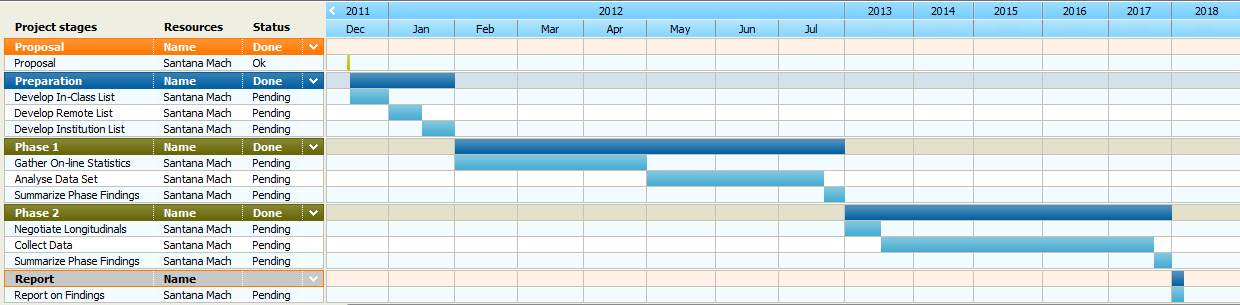
\includegraphics[width=1\textwidth]{Gantt.png}
  \end{center}
  \caption{Research Schedule}
  \label{fig:schedule}
\end{figure}

\end{document}
